\scanpage{67}

Un pantalon \inserted{(topologique)} subdivisé de façon standard, avec un ens $J$ de trous $(\operatorname{card}J=3)$ correspond à un ``triangle pondéré'' i.e.
\[
J\xrightarrow{\pi}\mathbb N
\qquad(\mathrm{NB}\ \pi(j)=\text{nb d'arêtes qui relient $j$ et $k$, $i\ne j\ne k$})
\]

Carte \inserted{\unsure{orientée|orienté}} découpée pantaloniquement, de façon standard $\Longleftrightarrow$ \deleted{\unsure{graphe}} un squelette pantalonique généralisé

\unsure{\deleted{(i.e. carte \unsure{cellulaire} (\unsure{pas néc. orientée}), dont les sommets marqués sont d'ordre $3$ (avec des sommets topologiques non marqués d'ordre $1$ éventuellement), et avec une pondération des \deleted{\unsure{arêtes orientées|arêtes repérées}} \inserted{drapeaux de \unsure{types|type} $0,1$} (sommet \inserted{marqué} et arête \unsure{incidente|incidents}) de telle façon que l'on ait pour chaque arête (cf ci-contre)}}

\figure{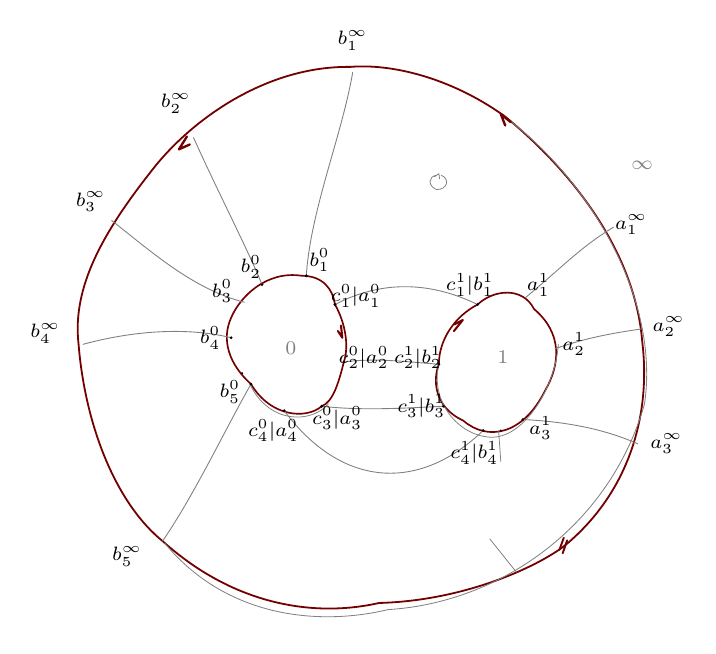
\begin{tikzpicture}[x=0.0028cm,y=-0.0028cm,line cap=round,line join=round,every node/.style={inner sep=1pt,font=\scriptsize}]
\draw[red!45!black,line width=.65pt] (1500,255) .. controls (1130,250) and (800,480) .. (620,700) .. controls (380,1000) and (240,1250) .. (270,1510) .. controls (300,1880) and (440,2230) .. (650,2400) .. controls (960,2680) and (1320,2750) .. (1630,2680) .. controls (2010,2670) and (2340,2520) .. (2470,2420) .. controls (2760,2180) and (2860,1830) .. (2820,1500) .. controls (2790,1120) and (2540,760) .. (2200,480) .. controls (1950,300) and (1680,240) .. (1500,255);
\draw[gray,line width=.3pt] (660,2410) .. controls (950,2760) and (1380,2780) .. (1670,2710) .. controls (2170,2680) and (2670,2340) .. (2830,1780) .. controls (2900,1310) and (2590,780) .. (2210,490);
\draw[red!45!black,line width=.6pt] (1280,1200) .. controls (1375,1200) and (1420,1260) .. (1430,1330) .. controls (1475,1410) and (1495,1515) .. (1470,1590) .. controls (1445,1690) and (1420,1770) .. (1370,1790) .. controls (1300,1850) and (1140,1840) .. (1050,1690) .. controls (950,1600) and (915,1490) .. (960,1390) .. controls (1000,1295) and (1120,1175) .. (1280,1200);
\draw[gray,line width=.28pt] (1045,1690) .. controls (1130,1870) and (1320,1870) .. (1400,1780);
\draw[red!45!black,line width=.6pt] (2075,1330) .. controls (2150,1260) and (2280,1250) .. (2330,1350) .. controls (2460,1460) and (2450,1600) .. (2380,1720) .. controls (2280,1920) and (2120,1950) .. (2010,1855) .. controls (1870,1790) and (1875,1660) .. (1900,1600) .. controls (1900,1490) and (1970,1385) .. (2075,1330);
\draw[gray,line width=.28pt] (1900,1600) .. controls (1860,1760) and (1980,1920) .. (2130,1930) .. controls (2290,1940) and (2430,1690) .. (2440,1510);
\draw[red!45!black,line width=.85pt] (2225,505)--(2180,468)--(2200,520);
\draw[red!45!black,line width=.85pt] (760,570)--(724,628)--(773,606);
\draw[red!45!black,line width=.75pt] (1457,1425)--(1463,1480)--(1443,1450);
\draw[red!45!black,line width=.75pt] (1968,1450)--(2008,1400)--(1970,1420);
\draw[red!45!black,line width=.7pt] (2465,2385)--(2445,2440) (2480,2397)--(2460,2455);
\draw[gray,line width=.32pt] (1510,280) .. controls (1460,570) and (1320,900) .. (1300,1200);
\draw[gray,line width=.32pt] (790,575) .. controls (900,820) and (1035,1080) .. (1100,1240);
\draw[gray,line width=.32pt] (420,950) .. controls (610,1100) and (790,1260) .. (1020,1320);
\draw[gray,line width=.32pt] (290,1510) .. controls (510,1450) and (755,1430) .. (960,1480);
\draw[gray,line width=.32pt] (650,2400) .. controls (800,2180) and (930,1900) .. (1050,1690);
\draw[gray,line width=.32pt] (1430,1330) .. controls (1650,1215) and (1870,1230) .. (2075,1330);
\draw[gray,line width=.32pt] (1470,1590) .. controls (1610,1570) and (1760,1590) .. (1900,1600);
\draw[gray,line width=.32pt] (1370,1790) .. controls (1540,1810) and (1730,1800) .. (1920,1790);
\draw[gray,line width=.32pt] (1200,1810) .. controls (1460,2160) and (1810,2180) .. (2100,1900);
\draw[gray,line width=.32pt] (2290,1300) .. controls (2460,1160) and (2540,1070) .. (2690,980);
\draw[gray,line width=.32pt] (2425,1530) .. controls (2570,1480) and (2680,1460) .. (2820,1440);
\draw[gray,line width=.32pt] (2280,1850) .. controls (2470,1860) and (2640,1890) .. (2800,1960);
\node[] at (1510,135) {$b_1^\infty$};
\node[] at (710,420) {$b_2^\infty$};
\node[] at (325,865) {$b_3^\infty$};
\node[] at (120,1460) {$b_4^\infty$};
\node[] at (490,2470) {$b_5^\infty$};
\node[] at (2770,970) {$a_1^\infty$};
\node[] at (2940,1430) {$a_2^\infty$};
\node[] at (2930,1960) {$a_3^\infty$};
\node[] at (1360,1130) {$b_1^0$};
\node[] at (1050,1160) {$b_2^0$};
\node[] at (920,1270) {$b_3^0$};
\node[] at (865,1480) {$b_4^0$};
\node[] at (955,1725) {$b_5^0$};
\node[] at (1525,1290) {$\unsure{c_1^0|a_1^0}$};
\node[] at (1560,1570) {$\unsure{c_2^0|a_2^0}$};
\node[] at (1440,1845) {$\unsure{c_3^0|a_3^0}$};
\node[] at (1150,1900) {$\unsure{c_4^0|a_4^0}$};
\node[] at (2040,1240) {$\unsure{c_1^1|b_1^1}$};
\node[] at (1805,1570) {$\unsure{c_2^1|b_2^1}$};
\node[] at (1820,1790) {$\unsure{c_3^1|b_3^1}$};
\node[] at (2060,2000) {$\unsure{c_4^1|b_4^1}$};
\node[] at (2350,1240) {$a_1^1$};
\node[] at (2510,1510) {$a_2^1$};
\node[] at (2360,1890) {$a_3^1$};
\node[text=gray] at (1230,1530) {$0$};
\node[text=gray] at (2190,1570) {$1$};
\node[text=gray] at (2820,700) {$\infty$};
\draw[gray,line width=.28pt] (1890,745) .. controls (1850,750) and (1850,795) .. (1890,810) .. controls (1940,810) and (1950,760) .. (1910,745) (1880,752)--(1900,738)--(1903,761);
\draw[gray,line width=.28pt] (2170,1900)--(2180,2040) (2130,2390)--(2250,2540);
\fill[black] (1010,1640) circle[radius=5];
\fill[black] (2180,1900) circle[radius=5];
\fill[black] (1300,1200) circle[radius=7];
\fill[black] (1100,1240) circle[radius=7];
\fill[black] (960,1480) circle[radius=7];
\fill[black] (1050,1690) circle[radius=7];
\fill[black] (1430,1330) circle[radius=7];
\fill[black] (1470,1590) circle[radius=7];
\fill[black] (1370,1790) circle[radius=7];
\fill[black] (1200,1810) circle[radius=7];
\fill[black] (2075,1330) circle[radius=7];
\fill[black] (1900,1600) circle[radius=7];
\fill[black] (1920,1790) circle[radius=7];
\fill[black] (2100,1900) circle[radius=7];
\fill[black] (2280,1850) circle[radius=7];
\end{tikzpicture}}

\figure{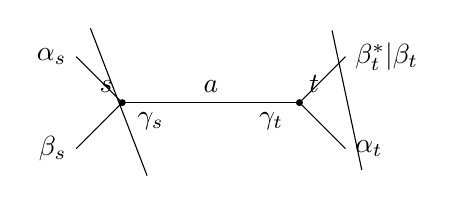
\begin{tikzpicture}[>=stealth,scale=.9]
\fill (0,0) circle (1.4pt) node[above left] {$s$};
\fill (2.5,0) circle (1.4pt) node[above right] {$t$};
\draw (0,0)--(2.5,0) node[midway,above] {$a$};
\draw (0,0)--(-.65,.65) node[left] {$\alpha_s$};
\draw (0,0)--(-.65,-.65) node[left] {$\beta_s$};
\draw (2.5,0)--(3.15,.65) node[right] {$\unsure{\beta_t^*|\beta_t}$};
\draw (2.5,0)--(3.15,-.65) node[right] {$\alpha_t$};
\node[below] at (.4,0) {$\gamma_s$};
\node[below] at (2.1,0) {$\gamma_t$};
% The diagram lies inside the subsequently cancelled block.
\draw (-.45,1.05)--(.35,-1.03);
\draw (2.96,1.02)--(3.38,-.95);
\end{tikzpicture}}
\[
\unsure{\deleted{\underbrace{\alpha_s+\beta_s}_{\unsure{\deleted{\alpha}\gamma'_s|\gamma'_s}}
=\underbrace{\unsure{\alpha_t^*+\beta_t^*|\alpha_t+\beta_t}}_{\gamma'_t}}}
\]

\unsure{\deleted{et $=$ la \uline{donnée} d'un \deleted{\unsure{isom|auto}} \inserted{anti-}isom des torseurs sous $\mathbb Z/\unsure{\gamma|\gamma_t}$ $(\gamma=\gamma'_s=\gamma'_t)$}
\[
\deleted{\substack{\text{somme circulaire}\\\text{de }[1,\alpha_s]\text{ et }[1,\beta_s]}
\ \simeq\
\substack{\text{somme}\\\text{circulaire}\\{}[1,\alpha_t]\text{ et }[1,\beta_t]}.}
\]}

\unsure{\figure{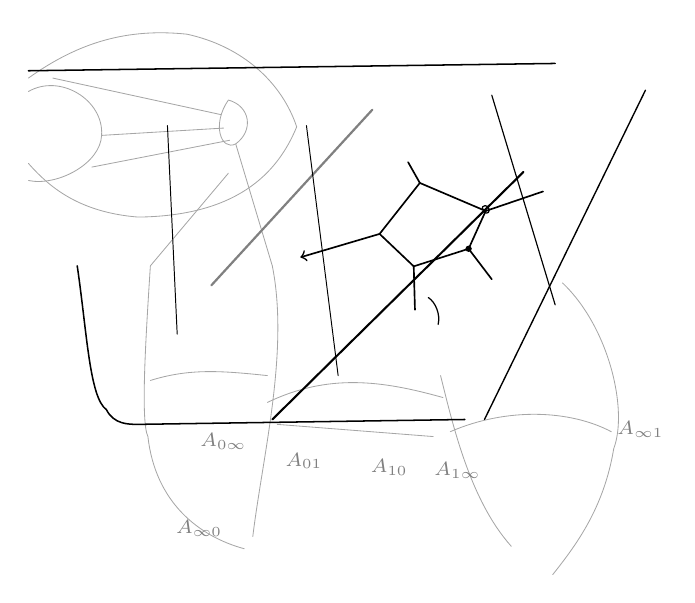
\begin{tikzpicture}[x=0.0031cm,y=-0.0031cm,line cap=round,line join=round,every node/.style={inner sep=1pt,font=\scriptsize}]
\draw[gray!70,line width=.3pt] (0,430) .. controls (210,280) and (410,225) .. (650,250) .. controls (880,300) and (1040,450) .. (1100,630) .. controls (1020,825) and (850,995) .. (450,1000) .. controls (200,980) and (80,870) .. (0,780);
\draw[gray!70,line width=.3pt] (0,485) .. controls (130,410) and (310,520) .. (300,665) .. controls (295,780) and (120,875) .. (0,850);
\draw[gray!70,line width=.3pt] (820,520) .. controls (910,545) and (925,645) .. (850,700) .. controls (790,730) and (750,620) .. (820,520);
\draw[gray!70,line width=.3pt] (100,430)--(790,580) (300,665)--(800,635) (260,795)--(825,685);
\draw[gray!70,line width=.3pt] (500,1200) .. controls (480,1510) and (460,1840) .. (490,1900) .. controls (520,2170) and (700,2310) .. (885,2360);
\draw[gray!70,line width=.3pt] (1000,1200) .. controls (1070,1550) and (960,1980) .. (920,2310);
\draw[gray!70,line width=.3pt] (1690,1650) .. controls (1740,1850) and (1810,2160) .. (1980,2350);
\draw[gray!70,line width=.3pt] (2190,1270) .. controls (2380,1450) and (2460,1790) .. (2400,1950) .. controls (2360,2190) and (2250,2340) .. (2150,2466);
\draw[gray!70,line width=.3pt] (500,1670) .. controls (660,1620) and (790,1630) .. (980,1650);
\draw[gray!70,line width=.3pt] (980,1760) .. controls (1230,1640) and (1450,1670) .. (1700,1740);
\draw[gray!70,line width=.3pt] (1020,1850)--(1660,1900);
\draw[gray!70,line width=.3pt] (1730,1880) .. controls (1960,1780) and (2220,1790) .. (2390,1880);
\draw[gray!70,line width=.3pt] (820,820)--(500,1200) (850,700)--(1000,1200);
\draw[black,line width=.6pt] (1605,860)--(1875,975)--(1805,1130)--(1580,1202)--(1440,1069)--(1605,860);
\draw[black,line width=.6pt] (1605,860)--(1557,775) (1875,975)--(2110,895) (1805,1130)--(1900,1255) (1580,1202)--(1585,1380);
\draw[black,line width=.6pt,->] (1440,1069)--(1115,1165);
\fill[black] (1805,1130) circle[radius=13];
\draw[black,line width=.45pt] (1865,970) .. controls (1850,950) and (1890,945) .. (1890,970) .. controls (1890,990) and (1865,987) .. (1865,970);
\draw[black,line width=.45pt] (1640,1330) .. controls (1670,1350) and (1690,1400) .. (1680,1440);
\draw[gray,line width=.8pt] (750,1280)--(1410,560);
\draw[black,line width=.75pt] (1000,1830)--(2030,815);
\draw[black,line width=.5pt] (2530,480)--(1870,1830);
\draw[black,line width=.42pt] (1900,500)--(2160,1360);
\draw[black,line width=.55pt] (200,1200) .. controls (240,1470) and (250,1740) .. (320,1790) .. controls (350,1850) and (410,1850) .. (450,1850) --(1790,1830);
\draw[black,line width=.55pt] (0,400)--(2160,370);
\draw[black,line width=.35pt] (570,625)--(610,1480) (1140,625)--(1270,1650);
\node[text=gray] at (800,1920) {$A_{0\infty}$};
\node[text=gray] at (1130,2000) {$A_{01}$};
\node[text=gray] at (1480,2025) {$A_{10}$};
\node[text=gray] at (1760,2040) {$A_{1\infty}$};
\node[text=gray] at (700,2275) {$A_{\infty0}$};
\node[text=gray] at (2510,1870) {$A_{\infty1}$};
\end{tikzpicture}}}
% crop-candidate: scan 67

\figure{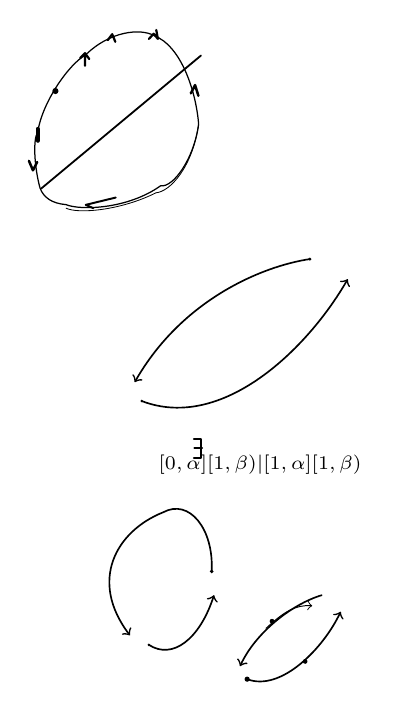
\begin{tikzpicture}[x=0.003cm,y=-0.003cm,line cap=round,line join=round,every node/.style={inner sep=1pt,font=\scriptsize}]
\draw[black,line width=.45pt] (130,740) .. controls (105,650) and (100,530) .. (120,505) .. controls (140,370) and (260,210) .. (320,180) .. controls (425,75) and (555,65) .. (610,95) .. controls (730,140) and (790,340) .. (800,470) .. controls (780,620) and (690,740) .. (640,730) .. controls (500,830) and (300,835) .. (240,810) .. controls (180,805) and (145,780) .. (130,740);
\draw[black,line width=.3pt] (800,470) .. controls (775,650) and (680,755) .. (620,760) .. controls (470,835) and (290,850) .. (240,825);
\draw[black,line width=.65pt] (135,742)--(810,180);
\draw[black,line width=1.5pt] (120,490)--(120,540);
\fill[black] (195,330) circle[radius=13];
\draw[black,line width=.8pt] (300,190)--(320,170)--(338,195) (320,180)--(320,223);
\draw[black,line width=.8pt] (416,115)--(435,90)--(448,122) (590,110)--(610,88)--(628,110)--(621,72);
\draw[black,line width=.9pt] (767,340)--(785,305)--(799,350) (83,625)--(100,665)--(118,630);
\draw[black,line width=.7pt] (450,780)--(323,811)--(355,825);
\draw[black,line width=.6pt,->] (1270,1040) .. controls (1070,1070) and (730,1210) .. (530,1560);
\draw[black,line width=.6pt,->] (560,1640) .. controls (900,1770) and (1260,1420) .. (1430,1125);
\fill[black] (1270,1040) circle[radius=7];
\fill[black] (560,1640) circle[radius=6];
\node[] at (1060,1910) {$\unsure{[0,\alpha][1,\beta)|[1,\alpha][1,\beta)}$};
\draw[black,line width=.7pt] (780,1800)--(810,1800)--(810,1880)--(780,1880) (782,1840)--(815,1840);
\draw[black,line width=.6pt,->] (855,2360) .. controls (865,2180) and (760,2050) .. (650,2110) .. controls (450,2190) and (335,2400) .. (510,2630);
\draw[black,line width=.6pt,->] (590,2670) .. controls (690,2735) and (805,2645) .. (865,2460);
\fill[black] (855,2360) circle[radius=8];
\fill[black] (590,2670) circle[radius=6];
\draw[black,line width=.6pt,->] (1320,2460) .. controls (1190,2500) and (1040,2620) .. (975,2760);
\draw[black,line width=.35pt,->] (1085,2600) .. controls (1160,2530) and (1210,2500) .. (1280,2505);
\draw[black,line width=.6pt,->] (1005,2815) .. controls (1150,2870) and (1330,2680) .. (1400,2530);
\fill[black] (1110,2570) circle[radius=10];
\fill[black] (1250,2740) circle[radius=10];
\fill[black] (1005,2815) circle[radius=11];
\end{tikzpicture}}

\figure{\begin{tikzpicture}[x=1cm,y=1cm]
% Pale earlier writing and dark replacements occupy the same area.
\node[gray,anchor=west] at (4.35,.47) {$\unsure{\alpha'=\dfrac{\alpha'+\beta'+\gamma'}2}$};
\node[gray,anchor=west] at (4.92,-1.05) {$\deleted{\unsure{\alpha}}$};
\node[gray,anchor=west,font=\small] at (5.18,-2.00) {$\unsure{\alpha=(\alpha+\beta+\gamma)-(\beta-\gamma)|\alpha=(\alpha'+\beta'-\gamma')-\deleted{(\beta-\gamma)}}\ \unsure{=}$};
\node[gray,anchor=west,font=\small] at (5.2,-3.05) {$\unsure{\dfrac{\alpha'+\beta'+\gamma'}2}$};
\draw[gray] (8.2,-2.34)--(9.85,-2.34);
\node[gray] at (9.8,-3.05) {$\unsure{\alpha'}$};
\node[anchor=west] at (0,0) {$\beta+\gamma=\alpha'$};
\node[anchor=west] at (0,-1.18) {$\gamma+\alpha=\beta'$};
\node[anchor=west] at (0,-2.4) {$\alpha+\beta=\gamma'$};
\node[anchor=west] at (4.05,0) {$\alpha=\dfrac{\beta'+\gamma'-\alpha'}2=\dfrac{\alpha'+\beta'+\gamma'}2-\alpha'$};
\node[anchor=west] at (4.05,-1.18) {$\beta=\dfrac{\gamma'+\alpha'-\beta'}2$};
\node[anchor=west] at (4.05,-2.4) {$\gamma=\dfrac{\alpha'+\beta'-\gamma'}2$};
\end{tikzpicture}}

{\color{gray}
\[
\begin{aligned}
&\unsure{2(\alpha+\beta+\gamma)-\alpha'=\beta'+\gamma'}\\
&\uline{2\alpha}+\beta+\gamma=\beta'+\gamma'\\
&\beta+\gamma=\alpha'
\end{aligned}
\]}

\figure{\begin{tikzpicture}[x=0.003cm,y=-0.003cm,line cap=round,line join=round,every node/.style={inner sep=1pt,font=\scriptsize}]
\draw[gray,line width=.4pt] (1250,220)--(530,1540) (480,1610)--(2015,1600)--(1255,230);
\node[] at (1250,110) {$0$};
\node[] at (360,1660) {$1$};
\node[] at (2160,1680) {$\infty$};
\node[] at (250,940) {$\gamma=4$};
\node[] at (2180,900) {$\beta=5$};
\node[] at (1250,2020) {$\alpha=3$};
\draw[black,line width=.65pt] (997,540)--(1043,566);
\node[] at (860,550) {$c_1$};
\draw[black,line width=.65pt] (907,780)--(953,806);
\node[] at (770,790) {$c_2$};
\draw[black,line width=.65pt] (827,970)--(873,996);
\node[] at (690,980) {$c_3$};
\draw[black,line width=.65pt] (727,1160)--(773,1186);
\node[] at (590,1170) {$c_4$};
\draw[black,line width=.65pt] (1505,657)--(1555,631);
\node[] at (1690,645) {$b_5$};
\draw[black,line width=.65pt] (1575,812)--(1625,786);
\node[] at (1760,800) {$b_4$};
\draw[black,line width=.65pt] (1675,992)--(1725,966);
\node[] at (1860,980) {$b_3$};
\draw[black,line width=.65pt] (1795,1232)--(1845,1206);
\node[] at (1980,1220) {$b_2$};
\draw[black,line width=.65pt] (1885,1382)--(1935,1356);
\node[] at (2070,1370) {$b_1$};
\draw[black,line width=.65pt] (875,1585)--(878,1640);
\node[] at (875,1740) {$a_1$};
\draw[black,line width=.65pt] (1210,1585)--(1213,1640);
\node[] at (1210,1740) {$a_2$};
\draw[black,line width=.65pt] (1510,1580)--(1513,1635);
\node[] at (1510,1735) {$a_3$};
\end{tikzpicture}}

\figure{\begin{tikzpicture}[x=0.0034cm,y=-0.0034cm,line cap=round,line join=round,every node/.style={inner sep=1pt,font=\scriptsize}]
\draw[gray,line width=.4pt] (950,220)--(325,1430) (300,1515) .. controls (850,1550) and (1260,1460) .. (1630,1495) (970,220) .. controls (1080,670) and (1440,1210) .. (1600,1410);
\node[] at (960,120) {$0$};
\node[] at (210,1530) {$1$};
\node[] at (1740,1540) {$\infty$};
\node[] at (970,1340) {$a_3$};
\node[] at (940,1560) {$a_2$};
\node[] at (940,1710) {$\unsure{a^1|a_1}$};
\node[] at (300,800) {$c_1$};
\node[] at (470,880) {$c_2$};
\node[] at (640,930) {$c_3$};
\node[] at (805,975) {$c_4$};
\node[] at (1080,970) {$b_5$};
\node[] at (1260,950) {$b_4$};
\node[] at (1440,890) {$b_3$};
\node[] at (1630,835) {$b_2$};
\node[] at (1830,785) {$b_1$};
\fill[black] (955,1005) circle[radius=7];
\draw[black,line width=.65pt] (1490,1735)--(1535,1825);
\end{tikzpicture}}

\figure{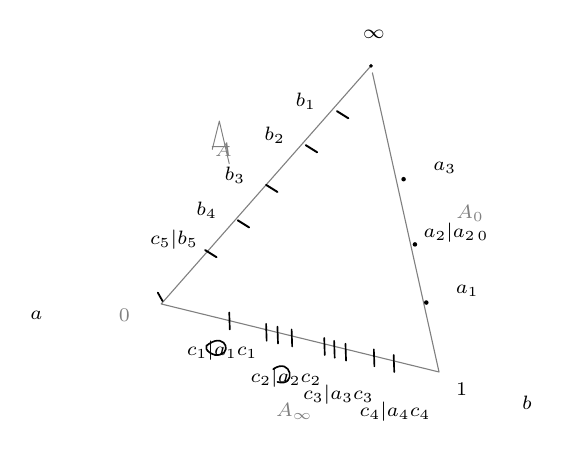
\begin{tikzpicture}[x=0.0036cm,y=-0.0036cm,line cap=round,line join=round,every node/.style={inner sep=1pt,font=\scriptsize}]
\draw[gray,line width=.4pt] (1350,180)--(610,1020)--(1590,1260)--(1355,205);
\fill[black] (1350,180) circle[radius=7];
\draw[black,line width=.65pt] (598,980)--(615,1010);
\node[] at (1360,70) {$\infty$};
\node[text=gray] at (480,1060) {$0$};
\node[] at (1670,1320) {$1$};
\node[] at (170,1060) {$a$};
\node[] at (1900,1370) {$b$};
\node[text=gray] at (1080,1400) {$\unsure{A_\infty}$};
\node[text=gray] at (830,475) {$\unsure{A}$};
\node[text=gray] at (1700,700) {$\unsure{A_0}$};
\draw[black,line width=.7pt] (1230,340)--(1270,365);
\node[] at (1120,305) {$b_1$};
\draw[black,line width=.7pt] (1120,460)--(1160,485);
\node[] at (1010,425) {$b_2$};
\draw[black,line width=.7pt] (980,600)--(1020,625);
\node[] at (870,565) {$\unsure{b_3}$};
\draw[black,line width=.7pt] (880,725)--(920,750);
\node[] at (770,690) {$b_4$};
\draw[black,line width=.7pt] (765,830)--(805,855);
\node[] at (655,795) {$\unsure{c_5|b_5}$};
\fill[black] (1465,580) circle[radius=8];
\node[] at (1610,540) {$a_3$};
\fill[black] (1505,810) circle[radius=8];
\node[] at (1650,770) {$\unsure{a_2|a_{2\,0}}$};
\fill[black] (1545,1015) circle[radius=8];
\node[] at (1690,975) {$\unsure{a_1}$};
\draw[black,line width=.6pt] (850,1050)--(852,1110);
\draw[black,line width=.6pt] (980,1090)--(982,1150);
\draw[black,line width=.6pt] (1020,1100)--(1022,1160);
\draw[black,line width=.6pt] (1070,1110)--(1072,1170);
\draw[black,line width=.6pt] (1185,1140)--(1187,1200);
\draw[black,line width=.6pt] (1220,1150)--(1222,1210);
\draw[black,line width=.6pt] (1260,1160)--(1262,1220);
\draw[black,line width=.6pt] (1360,1180)--(1362,1240);
\draw[black,line width=.6pt] (1430,1200)--(1432,1260);
\node[] at (825,1185) {$\unsure{c_1|\deleted{a_1}c_1}$};
\node[] at (1050,1280) {$\unsure{c_2|\deleted{a_2}c_2}$};
\node[] at (1235,1340) {$\unsure{c_3|\deleted{a_3}c_3}$};
\node[] at (1435,1400) {$\unsure{c_4|\deleted{a_4}c_4}$};
\draw[gray,line width=.35pt] (790,475)--(815,375)--(850,525) (790,465)--(850,465);
\draw[black,line width=.6pt] (780,1160) .. controls (840,1120) and (865,1205) .. (800,1200) .. controls (765,1190) and (760,1165) .. (780,1160) (1005,1250) .. controls (1070,1205) and (1090,1315) .. (1020,1295);
\end{tikzpicture}}

\uline{NB} $\alpha',\beta',\gamma'$ OK ssi $\alpha'+\beta'+\gamma'$ pair

\unsure{\figure{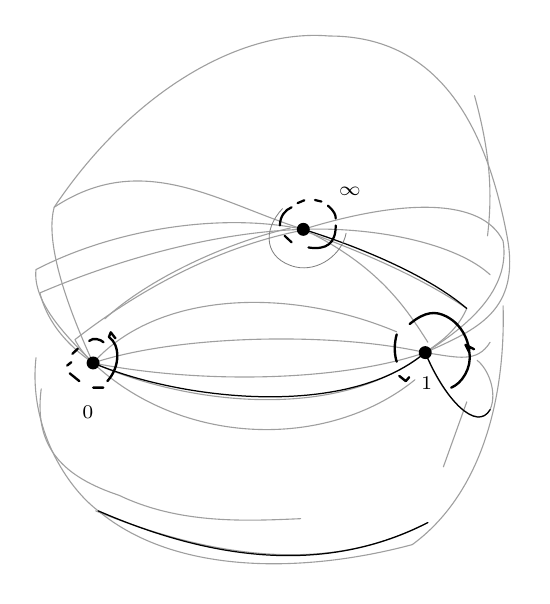
\begin{tikzpicture}[x=0.0033cm,y=-0.0033cm,line cap=round,line join=round,every node/.style={inner sep=1pt,font=\scriptsize}]
\draw[gray!75,line width=.4pt] (520,1370) .. controls (410,1130) and (335,900) .. (370,770) .. controls (660,335) and (1080,80) .. (1430,110) .. controls (1870,110) and (2040,485) .. (2115,880) .. controls (2170,1170) and (2000,1240) .. (1800,1330);
\draw[gray!75,line width=.4pt] (370,770) .. controls (710,545) and (1000,750) .. (1330,855);
\draw[gray!75,line width=.4pt] (1330,855) .. controls (1720,735) and (2020,735) .. (2100,900) .. controls (2130,1090) and (1960,1230) .. (1800,1330);
\draw[gray!75,line width=.4pt] (1330,855) .. controls (1020,790) and (610,850) .. (300,1010) .. controls (285,1140) and (430,1280) .. (520,1370);
\draw[gray!75,line width=.4pt] (1330,855) .. controls (1000,865) and (630,965) .. (315,1100) .. controls (350,1240) and (455,1325) .. (520,1370);
\draw[gray!75,line width=.4pt] (1320,860) .. controls (1020,920) and (720,1070) .. (450,1280) .. controls (470,1320) and (495,1345) .. (520,1370);
\draw[gray!75,line width=.4pt] (1280,850) .. controls (1040,905) and (740,1040) .. (565,1200);
\draw[gray!75,line width=.4pt] (1330,855) .. controls (1610,845) and (1920,910) .. (2050,1030);
\draw[gray!75,line width=.4pt] (1330,860) .. controls (1580,950) and (1800,1050) .. (1960,1160) .. controls (1920,1250) and (1855,1290) .. (1800,1330);
\draw[gray!75,line width=.4pt] (1370,875) .. controls (1630,1010) and (1730,1165) .. (1810,1290);
\draw[gray!75,line width=.4pt] (520,1370) .. controls (760,1100) and (1260,1070) .. (1690,1250);
\draw[gray!75,line width=.4pt] (520,1370) .. controls (850,1260) and (1450,1250) .. (1800,1330);
\draw[gray!75,line width=.4pt] (520,1370) .. controls (920,1450) and (1460,1445) .. (1800,1330);
\draw[gray!75,line width=.4pt] (520,1370) .. controls (880,1530) and (1460,1600) .. (1800,1330);
\draw[gray!75,line width=.4pt] (520,1370) .. controls (860,1690) and (1420,1710) .. (1760,1435);
\draw[gray!75,line width=.4pt] (300,1350) .. controls (270,1620) and (420,1850) .. (540,1940) .. controls (840,2190) and (1340,2180) .. (1750,2070) .. controls (2010,1880) and (2110,1520) .. (2100,1150);
\draw[gray!75,line width=.4pt] (320,1470) .. controls (290,1700) and (410,1810) .. (620,1880) .. controls (850,1990) and (1100,1980) .. (1320,1970);
\draw[gray!75,line width=.4pt] (530,1940) .. controls (1000,2130) and (1440,2180) .. (1810,1985);
\draw[gray!75,line width=.4pt] (1800,1330) .. controls (1870,1510) and (2000,1635) .. (2050,1550) .. controls (2080,1480) and (2040,1390) .. (2000,1360);
\draw[gray!75,line width=.4pt] (1800,1330) .. controls (1930,1350) and (2000,1370) .. (2050,1290);
\draw[gray!75,line width=.4pt] (1990,340) .. controls (2050,560) and (2060,710) .. (2040,880);
\draw[gray!75,line width=.4pt] (1960,1520)--(1870,1770);
\draw[black,line width=.45pt] (1330,855) .. controls (1570,930) and (1820,1040) .. (1960,1160);
\draw[black,line width=.45pt] (520,1370) .. controls (850,1510) and (1490,1590) .. (1800,1330);
\draw[black,line width=.45pt] (540,1940) .. controls (1000,2140) and (1430,2180) .. (1810,1985);
\draw[black,line width=.45pt] (1800,1330) .. controls (1880,1520) and (2000,1635) .. (2050,1550);
\draw[black,line width=.8pt] (1240,840) .. controls (1240,805) and (1260,780) .. (1285,770) (1308,754)--(1334,743) (1375,742)--(1400,748) (1425,764) .. controls (1450,785) and (1455,800) .. (1455,813) (1455,840) .. controls (1455,910) and (1420,935) .. (1350,925) (1285,905)--(1258,880);
\draw[gray,line width=.3pt] (1250,775) .. controls (1170,860) and (1180,970) .. (1300,1000) .. controls (1390,1020) and (1480,950) .. (1495,870);
\draw[black,line width=.85pt] (440,1335)--(461,1315) (420,1380)--(436,1367) (430,1410)--(467,1440) (520,1465)--(559,1465) (575,1440) .. controls (625,1385) and (625,1300) .. (581,1270) --(588,1252) --(606,1275) (505,1285) .. controls (520,1270) and (550,1280) .. (560,1290);
\draw[black,line width=.85pt] (1690,1260) .. controls (1680,1295) and (1680,1335) .. (1690,1365) (1700,1420)--(1725,1440)--(1738,1425) (1740,1220) .. controls (1800,1170) and (1840,1170) .. (1880,1190) .. controls (1950,1225) and (1970,1300) .. (1970,1330) (1970,1330)--(1955,1300)--(1988,1317) (1970,1330) .. controls (1980,1390) and (1940,1450) .. (1900,1465);
\fill[black] (1330,855) circle[radius=25];
\fill[black] (520,1370) circle[radius=25];
\fill[black] (1800,1330) circle[radius=25];
\node[] at (1510,710) {$\infty$};
\node[] at (500,1560) {$0$};
\node[] at (1805,1450) {$1$};
\end{tikzpicture}}}

\[
\begin{array}{l|l}
\text{trois sommets}&\text{\unsure{sommets|sommet} d'ordre }\alpha',\beta',\gamma'\\
\alpha+\beta+\gamma\ \text{\unsure{\deleted{bigones}\,arêtes|bigones}}&
\end{array}
\]
\deleted{$\unsure{\alpha+\beta+\gamma}$}
\[
\left\{\begin{array}{ll}
(\alpha-1)+(\beta-1)+(\gamma-1)&
\overbrace{\text{faces-bigones}}^{=\alpha+\beta+\gamma-2}\\
2&\text{faces-triangles}
\end{array}\right.
\quad\bigg|\quad \alpha+\beta+\gamma-1\ \text{faces}
\]

\mspage{66}
